\section{Zielsetzung}
In diesem Versuch werden Anwendungen eines Operationsverstärkers untersucht.
Dazu werden verschiedene Schaltungen mit Operationsverstärkern aufgebaut und ihre elektrotechnischen Eigenschaften geprüft.
Kenngrößen und Zusammenhänge werden vermessen und mit den Erwartungen eines idealen Operationsverstärkers verglichen.
 
\section{Theorie}
\label{sec:Theorie}
Der Operationsverstärker (\textit{OP}, \textit{OpAmp}) ist ein wichtiges Bauteil zur Verstärkung von Spannungssignalen.
Dem Aufbau eines OpAmp's liegt ein Differenzverstärker zur Grunde, weshalb auch die Differenz zweier anliegender Spannungssignale verstärkt wird.
Der invertierende Eingang wird mit einem \enquote{-} gekennzeichnet, der nicht-Invertierende mit einem \enquote{+}.
Ein idealer OpAmp hat eine unendliche Leerlaufverstärkung, wohingegen der reale Operationsverstärker einen Verstärkungsfaktor $V$ von etwa $10^4$ bis $10^7$ aufweist.
Der OpAmp wird mit zwei Betriebsspannungen $\pm U_\text{B}$ versorgt, wodurch die Amplitude des Ausgangsignals 
\begin{equation}
    U_\text{a} = V (U_+ - U_-)
    \label{eq:U_a}
\end{equation}
in den Bereich $-U_\text{B} < U_\text{a} < U_\text{B}$ eingeschränkt ist.
Dies kann auch anhand der Übertragungskennlinie eines idealen OpAmp's in \autoref{fig:Kennlinie} gesehen werden.
\begin{figure}
    \centering
    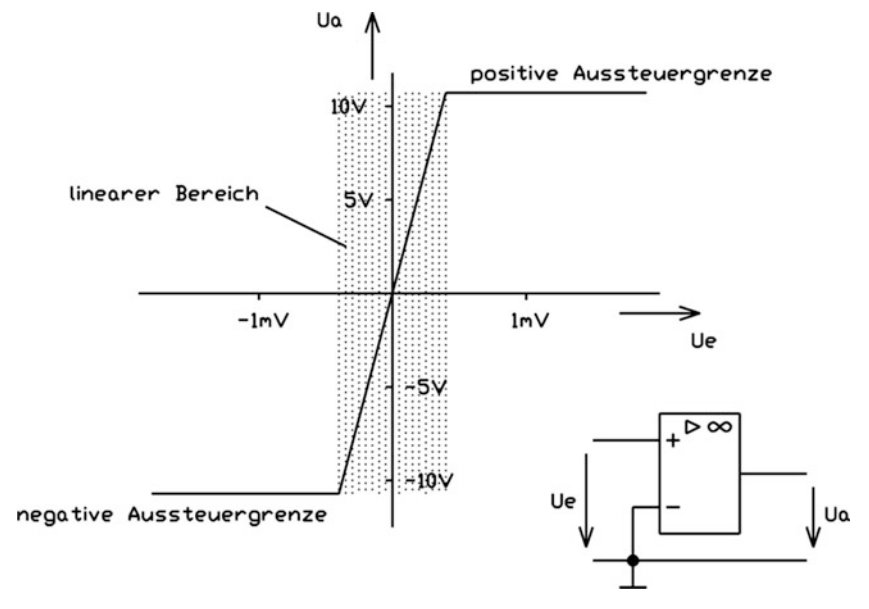
\includegraphics[width = .7\textwidth]{"content/pics/Kennlinie.png"}
    \caption{Übertragungskennlinie eines idealen Operationsverstärkers \cite{Federau2017}.}
    \label{fig:Kennlinie}
\end{figure}
Überschreitet die Verstärkung bei einem realen OpAmp die Betriebsspannung, so erreicht das Signal ein Plateau einige Volt (milli Volt) unter der Betriebsspannung.
Die Kennlinie eines realen Verstärkers kann außerdem um einen Offset $U_\text{offset}$ verschoben sein.

Beim idealen Operationsverstärker ist der Eingangswiderstand unendlich groß und der Ausgangswiderstand $\qty{0}{\ohm}$. Ein realer OpAmp hat typischerweise einen Eingangswiderstand
von $R_\text{e} > \qty{1}{\mega\ohm}$ und einen Ausgangswiderstand von etwa $R_\text{a} = \qtyrange[range-phrase = -]{10}{1000}{\ohm}$.
Ebenso hat der ideale OpAmp eine unendliche Übertragungsbandbreite, wohingegen der reale Operationsverstärker eine Grenzfrequenz zwischen $\qty{10}{\hertz}$ und 
$\qty{10}{\kilo\hertz}$ hat. Die Bandbreite wird bei Operationsverstärkern mit dem konstanten Verstärkung-Bandbreite-Produkt angegeben.
Des Weiteren tritt auch eine Gleichtaktverstärkung auf, also wenn gleiche Spannungssignale anliegen. Da dieses Verhalten unerwünscht ist, wird die Kenngröße der 
Gleichtaktunterdrückung $G$
\begin{equation}
    G = \frac{V_0}{V_\text{Gl}}
    \label{eq:Gleichtakt}
\end{equation}
als Verhältnis der Leerlaufverstärkung $V_0$ und der Gleichtaktverstärkung $V_\text{Gl}$ angegeben.

\subsection{Grundlegende Schaltungen}
Durch Rückkopplung des Ausgangsignals auf den Eingang (Feedback) kann ein Operationsverstärker in vielen Schaltunge mit unterschiedlichen Funktionen verwendet werden.
Eine positive Rückkopplung verstärkt dabei das Eingangssignal, während negatives Feedback dem Eingangssignal entgegen wirkt.
Durch zweiteres kann eine Stabilisierung des Betriebs des OpAmp's erreicht werden.

\subsubsection{Invertierender Linearverstärker}
Bei einem invertierenden Verstärker wird eine Rückkopplung des Ausgangsignals auf den invertierenden Eingang (Gegenkopplung) gegeben.
\begin{figure}
    \centering
    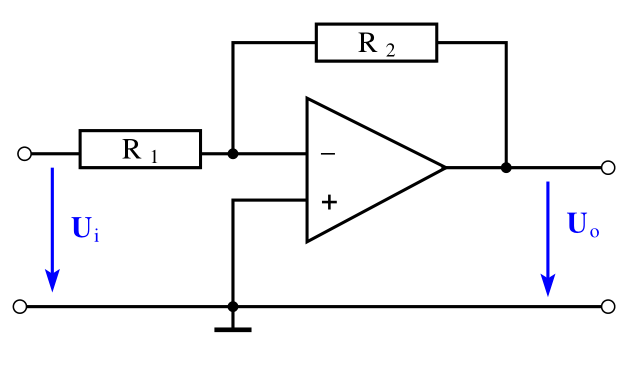
\includegraphics[width = .5\textwidth]{"content/pics/inverting.png"}
    \caption{Schaltplan eines invertierenden Linearverstärkers \cite{v51}.}
    \label{fig:inverting}
\end{figure}
Nach \autoref{eq:U_a} gilt mit $U_0 \equiv U_\text{a}$ 
\begin{equation*}
U_i = -\frac{U_\text{a}}{V}.
\end{equation*}
Mit der Kirchhoffschen Knotenregel gilt für den Knoten vor dem invertierenden Eingang 
\begin{equation*}
    \frac{U_i - U_1}{U_\text{a} - U_1} = \frac{R_1}{R_1 + R_2}\;.
\end{equation*}
Daraus folgt für die Verstärkung 
\begin{align}
    \frac{1}{V'} &= -\frac{U_1}{U_\text{a}} = \frac{1/V} + \frac{R_1}{R_2}\left(1 + \frac{1}{V}\right) \nonumber \\
    \Leftrightarrow V' &\approx \frac{R_2}{R_1} \left( = \frac{U_\text{a}}{U_\text{e}}\right) \;,
    \label{eq:invert}
\end{align}
da $V \gg 1$ ist.
Die Bandbreite des Verstärkers wird um den Faktor 
\begin{equation}
    g := \frac{V}{V'}
\end{equation}
erhöht.

\subsubsection{Integrator}
Der Schaltplan eines Integrators ist in \autoref{fig:integrator} gegeben.
\begin{figure}
    \centering
    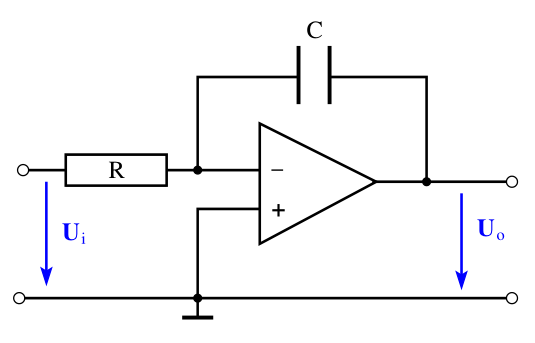
\includegraphics[width = .5\textwidth]{"content/pics/integrator.png"}
    \caption{Schaltplan eines Integrators \cite{v51}.}
    \label{fig:integrator}
\end{figure}
Hier gilt für den Knotenpunkt 
\begin{equation*}
    I_1 + I_\text{C} = 0
\end{equation*}
und mit  
\begin{equation*}
    I_1 = \frac{U_1}{R}
\end{equation*}
und 
\begin{equation*}
    \int I_C \symup{d}t = Q = CU_\text{a}
\end{equation*}
für die Ausgangsspannung 
\begin{equation}
    U_\text{a} = -\frac{1}{RC} \int U_1 \symup{d}t \;.
    \label{eq:integrator1}
\end{equation}
Für eine Wechselspannung $U_1 = U_0 \symup{sin}\left(\omega t\right)$ ist also 
\begin{equation}
    U_\text{a} = \frac{U_0}{\omega RC} \symup{cos}\left(\omega t\right) \;.
    \label{eq:integrator2}
\end{equation}

\subsubsection{Differenzierer}
Beim Differenzierer (\autoref{fig:differenzierer}) sind Widerstand und Kondensator getauscht.
\begin{figure}
    \centering
    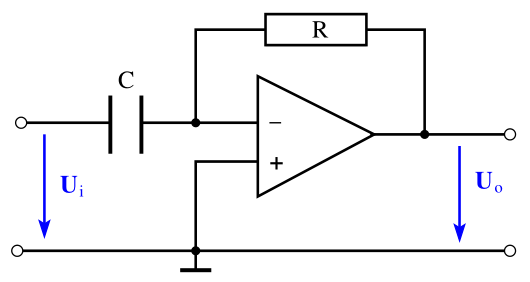
\includegraphics[width = .5\textwidth]{"content/pics/differenzierer.png"}
    \caption{Schaltplan eines Differenzierers \cite{v51}.}
    \label{fig:differenzierer}
\end{figure}
Analog zum Integrator folgt mit 
\begin{equation*}
    I_1 = \dot{Q} = C \dot{U}_1
\end{equation*}
\begin{equation}
    U_\text{a} = -RC \cdot \dot{U}_1 \;.
    \label{eq:differenzierer1}
\end{equation}
Also mit einer sinusförmigen Wechselspannung
\begin{equation}
    U_\text{a} = -\omega RC U_0 \cdot \symup{cos}\left(\omega t\right) \;.
    \label{eq:differenzierer2}
\end{equation}
\subsubsection{Schmitt-Trigger}
Bei der Schaltung für den Schmitt-Trigger (\autoref{fig:schmitt_trigger}) wird nun eine Rückkopplung auf den nicht-invertierenden Eingang gegeben.
Dadurch springt das Signal des Verstärkers schalgartig auf seinen maximalen Wert $(-) U_\text{B}$, wenn eine gewisse Schwellenspannung überschritten (unterschritten) wird.
Der Schmitt-Trigger fungiert also als Schalter.
Die Schwellenspannung ist dabei durch 
\begin{equation}
    U_{\pm} = \pm \frac{R_1}{R_2} U_\text{B}
    \label{eq:schmitt_trigger}
\end{equation}
gegeben.
\begin{figure}
    \centering
    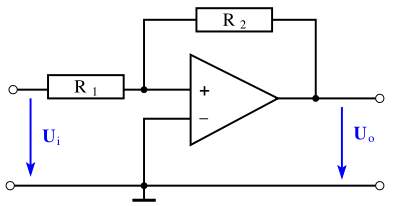
\includegraphics[width = .5\textwidth]{"content/pics/schmitt_trigger.png"}
    \caption{Schaltplan eines Schmitt-Triggers \cite{v51}.}
    \label{fig:schmitt_trigger}
\end{figure}

\subsubsection{Generator}
Zuletzt werden die Schaltungen eines Generators (\autoref{fig:generator1}) und eines Generators mit variierender Amplitude (\autoref{fig:generator2}) betrachtet.
\begin{figure}
    \centering
    \begin{subfigure}{\textwidth}
        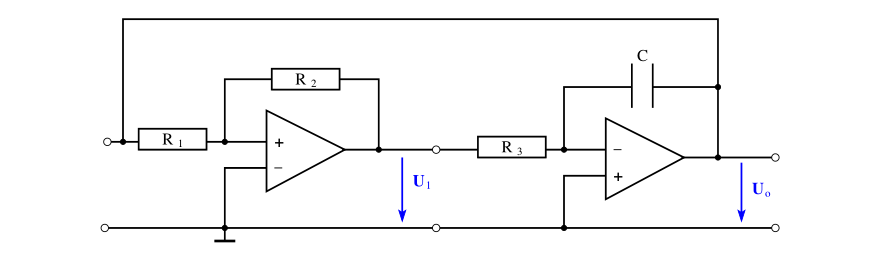
\includegraphics[width=\textwidth]{"content/pics/generator1.png"}
        \caption{Generator.}
        \label{fig:generator1}
    \end{subfigure}
    \vfill
    \begin{subfigure}{0.9\textwidth}
        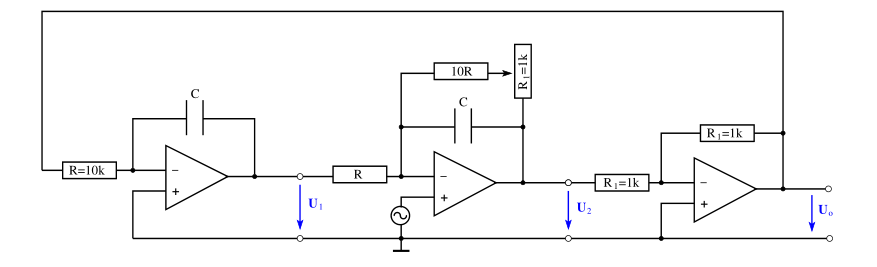
\includegraphics[width=\textwidth]{"content/pics/generator2.png"}
        \caption{Generator mit variierender Amplitude.}
        \label{fig:generator2}
    \end{subfigure}
    \caption{Schaltplan eines Generators und eines Generators mit variierender Amplitude \cite{v51}.}
    \label{fig:generator}
\end{figure}
Der Generator besteht aus einem Schmitt-Trigger und einem Integrator. Der Schmitt-Trigger schaltet bei jedem überschreiten oder unterschreiten des Schwellenwertes $U_{\pm}$
zwischen $\pm U_\text{B}$. Es liegt also eine Rechteckspannung an seinem Ausgang an. Am Ausgang des Integrators liegt dann eine Dreieckspannung an, die wieder auf den Eingang des 
Schmitt-Triggers rückgekoppelt wird. 
Die Frequenz des Generators ist durch
\begin{equation}
\nu_\text{a} = \frac{R_2}{4C R_1 R_3}
\label{eq:freq_generator}
\end{equation}
und die Amplitude durch 
\begin{equation}
    U_0 = U_\text{max} \frac{R_1}{R_2}
\end{equation}
gegeben. \\
Die Ausgangsspannung des Generators mit variierender Amplitude wird über die Differentialgleichung einer gedämpften Schwingung
\begin{equation}
    \frac{\symup{d}^2 U_\text{a}}{\symup{d}t^2} - \frac{\eta}{10RC}\frac{\symup{d}U_\text{a}}{\symup{d}t} + \frac{1}{(RC)^2}U_\text{a} = 0
\end{equation}
beschrieben. Die Konstante $-1 \leq \eta \leq 1$ ist dabei über $R_1$ einstellbar. 
Für $\eta < 0$ kann eine gedämpfte Schwingung gemessen werden, für $\eta > 0$ oszilliert das System.
Die Schwingungsdauer ist dabei 
\begin{equation}
    T = 2 \pi RC 
    \label{eq:T}
\end{equation}
und die Zerfallskonstante lautet
\begin{equation}
    \tau = \frac{20 RC}{|\eta|} \; .
\end{equation}
